\chapter*{Solucions}

\fontsize{11}{11.5}

\section*{TEMA \ref{chap:real}: \nameref{chap:real}}

\subsection*{Solucions als problemes clau \simbolclau}

 
\begin{enumerate}
	\item[\clauref{t1-r1}] 
	\begin{tasks}(4)
	\task $\sqrt[{6}]{5} $  \task  $\sqrt[{8}]{8} $  \task  $\sqrt[{8}]{x^{7} } $
	\end{tasks}
	
	\item[\clauref{t1-r2}] 
	\begin{tasks}(4)
\task  $2\sqrt[{}]{2} $    \task  $9\sqrt[{}]{3} $    \task  $\sqrt[{3}]{6} $   \task  $2\sqrt[{4}]{2} $   \task $\sqrt[{3}]{3} $    \task  $\sqrt[{3}]{49} $       \task  $\sqrt[{8}]{7} $    \task  $\sqrt[{}]{2} $
\end{tasks}
	
	\item[\clauref{t1-r3}] 
	\begin{tasks}(4)
	\task  $\sqrt[{4}]{2^{3} } =\sqrt[{12}]{2^{9} } $      \task  $\sqrt{7} =\sqrt[{16}]{7^{8} } $    \task  $\sqrt[{4}]{a^{6} } =\sqrt{a^{3} } $      \task  $\sqrt[{6}]{5^{12} } =\sqrt[{3}]{5^{6} } =5^{2} $
\end{tasks}

	\item[\clauref{t1-r4}]
	\begin{tasks}(4)
		 \task  $\sqrt[{3}]{5/4} $       \task  $\sqrt[{12}]{2^{3} \cdot 3} $    \task  $\sqrt[{12}]{5^{7} } $     \task  $2^{3} $      \task  $2^{4} \cdot \sqrt[{5}]{2^{4} } $     \task  $\sqrt[{}]{5} $      \task  3      \task  $5^{2} $
	\end{tasks}
	
	\item[\clauref{t1-r5}]
	\begin{tasks}(4)
	  \task  $15\sqrt[{}]{11} $  \task  $6\sqrt[{3}]{2} $     \task  $-\sqrt[{}]{6} /5$     \task  $-14\sqrt[{4}]{2} /3$      \task  $41\sqrt[{}]{3} /15$    \task  $13\sqrt[{}]{2} /5$
\end{tasks}
	
	\item[\clauref{t1-r9}] $(2+a)^{2} +4(2+a)\sqrt{a} +4a$
	
	
	\item[\clauref{t1-r6}]  
	\begin{tasks}(4)
	\task  $\frac{\sqrt[{3}]{3^{2} } }{3} $ \task  $\frac{3}{4} \, \sqrt[{4}]{2^{3} } $ \task  $3(\sqrt{2+1} )$ \task  $3+2\sqrt{2} $  \task  $(\sqrt{10} -\sqrt{6} )/2$   \task  $-(9+4\sqrt{5} )$
\end{tasks}
	
	\item[\clauref{t1-r8}] 
	\begin{tasks}(4)
	\task  $3\sqrt{6} $     \task  $\frac{\sqrt[{4}]{2^{3} } }{2} $    \task  $\frac{\sqrt{3} }{2} $    \task  35     \task  $2^{-64/15} $   \task  $33/4-5\sqrt{2} $    \task  39/56
\end{tasks}
\end{enumerate}


\subsection*{Solucions de l'autoavaluació}

\begin{tasks}[style=enumerate,label-width=4ex](4)
	\task c)
	\task c)
	\task d)
	\task a)
	\task c)
	\task $\dfrac{5\sqrt{15}-16}{7}$
	\task d)
\end{tasks}

%%%%%%%%%%%%%%%%%%%%%%%%%%%%%%%%%%%%%%%%%%%%%%%%%%%%%%%%%%%%%%%%%%%%%%%%%%%%%%%%%%%%%%%%%%%%%%%%%%%%%%%%%%%%%%%%%%%%%%%%%%%%%
%%%%%%%%%%%%%%%%%%%%%%%%%%%%%%%%%%%%%%%%%%%%%%%%%%%%%%%%%%%%%%%%%%%%%%%%%%%%%%%%%%%%%%%%%%%%%%%%%%%%%%%%%%%%%%%%%%%%%%%%%%%%%
%%%%%%%%%%%%%%%%%%%%%%%%%%%%%%%%%%%%%%%%%%%%%%%%%%%%%%%%%%%%%%%%%%%%%%%%%%%%%%%%%%%%%%%%%%%%%%%%%%%%%%%%%%%%%%%%%%%%%%%%%%%%%

\section*{TEMA \ref{chap:algebra}: \nameref{chap:algebra}}

\subsection*{Solucions als problemes clau \simbolclau}

\begin{enumerate}
 	\item[\clauref{t2-r10}] 
 	\begin{tasks}(2)
 	\task \textit{Q(x)=3x${}^{3}$+4x${}^{2}$-x+2; R(x)=-4}               \task \textit{Q(x)=2x+2;  R(x)=2x-1}         \task \textit{Q(x)=a(x${}^{3}$+ x${}^{2}$+ x+ 1); R(x)=a+b}       \task\textit{ Q(x)=x${}^{8}$+ x${}^{6}$+ x${}^{4}$+ x${}^{2}$+ 1; R(x)=0}
	 \end{tasks}

 	\item[\clauref{t2-r11}] 
 	\begin{tasks}(3)
 	\task \textit{3(x+2)·(x+1)}   \task \textit{x${}^{3}$(x+3)(x-3)}     \task \textit{4(x+3)(x+1)(x-1)}     \task \textit{-2(x+1)${}^{2}$·(x-3)}        \task \textit{x(x${}^{3}$-x${}^{2}$+8x-4)}    \task (\textit{x+1)${}^{2}$·(x-2)}     \task \textit{2(x+1)(x-2)(x-5)}       \task \textit{x${}^{2}$(x+1)(x-3)}         \task \textit{(x+4)(x+1)(x-2)}
 	 \end{tasks}
  
 	\item[\clauref{t2-r13}] 
 	\begin{tasks}(4)
 	\task $\frac{x-1}{3x(x+2)} $  \task $\frac{2(x+5)}{(x+1)^{2} } $   \task  $\frac{x-1}{x(x+2)} $   \task \textit{No es pot}   \task $\frac{(x^{2} +x+1)(x-1)}{x^{} } $           \task $\frac{1}{x+2} $        \task $\frac{x+2}{x-1} $       \task $\frac{2(x^{4} -x^{3} +x^{2} -x+1)}{x} $
 	 \end{tasks}
  
 	\item[\clauref{t2-r12}] 
 	\begin{tasks}(4)
 	\task $\frac{-4x}{(x+1)(x-1)} $  \task $\frac{-2}{x+1} $   \task  $\frac{-1}{x-1} $   \task $\frac{-2t+3}{t(t+2)} $  \task  0    \task $\frac{1-x^{2} }{x^{2} } $  \task $\frac{3x^{2} +5}{x(x+1)^{2} } $
 	 \end{tasks}
 	
 	\item[\clauref{t2-r14}] 
 	\begin{tasks}(4)
 	\task x=1, 2, -2       \task x=0, 5, -5            \task  x=1, -2        \task x=2, 3, -1, -2 \task x=1, 3, 5, -4
 	\task x=1                 \task x=-2, -1, 2            \task x=-3, -1, 2   \task x=-2, 2, 4                   \task x=-3, -2, 1      \task x=-3, 3, -2, 2  \task x=-1, 0, 5
 	 \end{tasks}
  
 	\item[\clauref{t2-r14b}]
 	
 	\begin{tasks}(4)
 	 \task x= 2/3,  -1/2 \task x=2, 1/7 \task x=2, -3/5     \task $(1\pm \sqrt{41} )/4$ 
 	 \end{tasks}
  
 	\item[\clauref{t2-r15}]
 	\begin{tasks}(4)
 	 \task x=4    \task x=4    \task x=9   \task x=7   \task x=2    \task x=38414   \task x=10    \task x=3    \task x=11        \task x=29  \task x=14  \task  x=1
 	 \end{tasks}
  
 	\item[\clauref{t2-r16}]
 	\begin{tasks}(4)
 	 \task x=1; y=16     \task x=6; y=8     \task x=10; y=2     \task x=4; y=7    \task x=3; y=1   \task  x=-2; y=8
 	 \end{tasks}
  
 	\item[\clauref{t2-key36}]
 	\begin{tasks}(2)
 	 \task x=7; y=2; z=11 
 	 \task x=4; y=-3; z=0 
 	 \task x=-1; y=4; z=4 
 	 \task x=8; y=4; z=-3 
 	 \end{tasks}

 	 \item[\clauref{t2-key37}]
 	\begin{tasks}(2)
 	 \task x=1; y=-5; z=4 
 	 \task x=-1; y=-2; z=-2 
 	 \task x=15; y=2; z=1 
 	 \task x=3; y=4; z=9 
 	 \end{tasks}

 	 \item[\clauref{t2-key38}]
 	 \begin{tasks}(2)
 	 \task x=1; y=-2; z=3 
 	 \task x=4; y=2; z=-3 
 	 \task x=1; y=-1; z=0 
 	 \task x=2; y=1/5; z=-1 
 	 \end{tasks}

 	 \item[\clauref{t2-key43}]
 	 \begin{tasks}(2)
 	 \task S.C.D. x=3/2; y=1/2; z=2 
 	 \task S.I. no té solució. 
 	 \task S.C.I. x=5-5z; y=2z-3; z=z 
 	 \task S.C.D. x=2; y=1/2; z=3/2
 	 \task S.I. no té solució.
 	 \task S.C.I. x=1-3y; y=y; z=3-7y
 	 \end{tasks}
\end{enumerate}

\subsection*{Solucions de l'autoavaluació}
\begin{tasks}[style=enumerate,label-width=4ex](4)
	\task c)
	\task c)
	\task No. Només 0, 2 o 4
	\task c)
	\task b)
	\task a)
	\task d)
	\task b)
	\task F, V, F, F
\end{tasks}
 


%%%%%%%%%%%%%%%%%%%%%%%%%%%%%%%%%%%%%%%%%%%%%%%%%%%%%%%%%%%%%%%%%%%%%%%%%%%%%%%%%%%%%%%%%%%%%%%%%%%%%%%%%%%%%%%%%%%%%%%%%%%%%
%%%%%%%%%%%%%%%%%%%%%%%%%%%%%%%%%%%%%%%%%%%%%%%%%%%%%%%%%%%%%%%%%%%%%%%%%%%%%%%%%%%%%%%%%%%%%%%%%%%%%%%%%%%%%%%%%%%%%%%%%%%%%
%%%%%%%%%%%%%%%%%%%%%%%%%%%%%%%%%%%%%%%%%%%%%%%%%%%%%%%%%%%%%%%%%%%%%%%%%%%%%%%%%%%%%%%%%%%%%%%%%%%%%%%%%%%%%%%%%%%%%%%%%%%%%

\section*{TEMA \ref{chap:trig}: \nameref{chap:trig}}
\subsection*{Solucions als problemes clau \simbolclau}
\begin{enumerate}
	\item[\clauref{trig:ex16}] \begin{tasks}(2) \task $\hat C=33$; $b=26,8$; $c=17,4$. \task  $\hat B=67$; $b=66,3$; $c=28,1$. \task  $\hat C=39$; $\hat B=51$; $a=396,7$. \task  $\hat B=58$; $b=56,01$; $a=66,05$    \end{tasks}
	\item[\clauref{trig:ex17}] $a=3,46$; $b=1,73$
	\item[\clauref{trig:ex18}] $\alpha=25,5^\circ$
	\item[\clauref{trig:ex19}] $a=25$; $c=20$; $\hat B=36,87^\circ$; $\hat C=53,13^\circ$
	\item[\clauref{trig:ex40}] \begin{tasks}(2) 
		\task $A=24.52$, $C=125.38$, $c=9.78$
		\task $B=75$, $a=14.64$, $c=17.93$
		\task No existeix cap triangle
		\task $A=77.36$, $B=C=51.32$ 
		\task*(2) Solució 1: $B=62.1$, $C=72.9$, $c=54.1$. Solució 2: $B=17.1$, $C=117.9$, $c=50$.
	\end{tasks}
	\item[\clauref{t3-r5}] d=35,49 km 
	\item[\clauref{t3-r6}] AB=24 km
	\item[\clauref{t3-r9}] cim A=827 m, cim B=751 m, distància entre cims AB=1687,3 m
\end{enumerate}

\subsection*{Solucions de l'autoavaluació}
\begin{enumerate} 
	\item a) $\sin(-750^\circ)=1/2$; \quad b) $\tg 570^\circ=\frac{-1}{\sqrt 3}=-\frac{\sqrt 3}{3}$;  \quad 
	c)  $\cos 20\pi/3 = -1/2$
	
	\item $\sin(105)=\sin(60+45)=\frac{\sqrt{6}+\sqrt{2}}{4}$,\quad
	$\cos(75)=\sin(30+45)=\frac{\sqrt{6}-\sqrt{2}}{4}$
	
	\item $c=17,32$, $\hat B=90^\circ$, $\hat C=60^\circ$
	\item Sí ho aconseguirà. Estan a 105,83 m.
	\item $\sin a=\frac{-1}{\sqrt 5}=-\frac{\sqrt 5}{5}$;\quad
	      $\cos a=\frac{-2}{\sqrt 5}=-\frac{2\sqrt 5}{5}$;
	\item a) $x=\left\{\begin{array}{l} 120 + n 360 \\ 240 +n 360 \end{array}\right.$,  \quad b) $x=45 + n 180$
	\item a) $(60+360k,120–360k)$, $(120+360k,60–360k)$;
	
	  b) $(75+360k, 15–360k)$, $(15+360k, 75–360k)$
	
	\item Sustituir el $\sin(2a)$ pel seu valor i aplicar  que $1–\cos 2a$ és el sinus al quadrat.
	
	\item perímetre = $300\cdot \sin 36^\circ = 176,3355$ m.; \quad àrea = 713,292 m$^2$.
	
	\item $8,63^\circ$
 
\end{enumerate}

%%%%%%%%%%%%%%%%%%%%%%%%%%%%%%%%%%%%%%%%%%%%%%%%%%%%%%%%%%%%%%%%%%%%%%%%%%%%%%%%%%%%%%%%%%%%%%%%%%%%%%%%%%%%%%%%%%%%%%%%%%%%%
%%%%%%%%%%%%%%%%%%%%%%%%%%%%%%%%%%%%%%%%%%%%%%%%%%%%%%%%%%%%%%%%%%%%%%%%%%%%%%%%%%%%%%%%%%%%%%%%%%%%%%%%%%%%%%%%%%%%%%%%%%%%%
%%%%%%%%%%%%%%%%%%%%%%%%%%%%%%%%%%%%%%%%%%%%%%%%%%%%%%%%%%%%%%%%%%%%%%%%%%%%%%%%%%%%%%%%%%%%%%%%%%%%%%%%%%%%%%%%%%%%%%%%%%%%%


\section*{TEMA \ref{chap:complex}: \nameref{chap:complex}}
\subsection*{Solucions als problemes clau \simbolclau}
\begin{enumerate}
	 \item[\clauref{t4_key2}]  
	 \begin{tasks}(4)
	    \task $5 -9i$
	    \task $-6-15i$
	    \task $-13+11i$
	 	\task 0
	 	\task 13
	 	\task $4 + 10i$
	 	\task $2i$
	 	\task $-4$
	 \end{tasks}
 
  \item[\clauref{t4_key3}]  
 \begin{tasks}(4)
 	\task $-{{1}\over{10}}-{{7\,i}\over{10}}$
 	\task $-{{11}\over{6}}+{{i}\over{2}}$
 	\task ${{2}\over{5}}-{{i}\over{5}}$
 	\task ${{34\,i}\over{5}}$
 \end{tasks}
 
 \item[\clauref{t4_key5}]  
 \begin{tasks}(2)
 	\task $|z|=2$,  $arg(z)=-30^\circ$
 	\task $|z|=\sqrt{8}$,  $arg(z)=225 = - 135^\circ$
 	\task $|z|=2$,  $arg(z)=-60^\circ$
 	\task $|z|=4$,  $arg(z)=-90^\circ$
 \end{tasks}

\item[\clauref{t4_key10}]  
 \begin{tasks}(2)
 	\task $2_{\, 60^\circ}= 1 - \sqrt{3} i$
 	\task $3_{\, -45^\circ}= \frac{3\sqrt{2}}{2} - \frac{3\sqrt{2}}{2} i$
 	\task $1_{\, 90^\circ}= i $
 	\task $5_{\, 120^\circ}= -\frac{5}{2} + i \frac{5\sqrt{3}}{2}$
 \end{tasks}
\end{enumerate}

\subsection*{Solucions de l'autoavaluació}
\begin{tasks}[style=enumerate,label-width=4ex](4)
	\task c)
	\task d)
	\task a)
	\task d)
	\task a)
	\task b)
	\task c)
\end{tasks}


%%%%%%%%%%%%%%%%%%%%%%%%%%%%%%%%%%%%%%%%%%%%%%%%%%%%%%%%%%%%%%%%%%%%%%%%%%%%%%%%%%%%%%%%%%%%%%%%%%%%%%%%%%%%%%%%%%%%%%%%%%%%%
%%%%%%%%%%%%%%%%%%%%%%%%%%%%%%%%%%%%%%%%%%%%%%%%%%%%%%%%%%%%%%%%%%%%%%%%%%%%%%%%%%%%%%%%%%%%%%%%%%%%%%%%%%%%%%%%%%%%%%%%%%%%%
%%%%%%%%%%%%%%%%%%%%%%%%%%%%%%%%%%%%%%%%%%%%%%%%%%%%%%%%%%%%%%%%%%%%%%%%%%%%%%%%%%%%%%%%%%%%%%%%%%%%%%%%%%%%%%%%%%%%%%%%%%%%%


\section*{SÍNTESI DE LA PART I - Àlgebra i Trigonometria}
\begin{enumerate}
\item a) $a\sqrt{a}$ \quad \quad b) $\frac{3\sqrt{2}-4\sqrt{6}}{6}$

\item a) $a\,\sqrt[20]{a}$ \quad \quad b)$\frac{2\sqrt{3}+3\sqrt{2}-6}{6}$

\item $x^2 (x+1) (x-2) (3x-1)$

\item 2

\item $x=3$ vàlida.

\item $x=1$

\item $(3, +\infty)$

\item $x=2$, $y=-1$, $z=2$

\item S.C.I. $x=1$, $y=z-3$, $z=z$

\item Els costats són 10.49 cm i 20.25 cm, el perímetre 61.48 cm. L'àrea 83.23 cm$^2$.

\item Primer obtenim els costats resolent un sistema d'equacions $a=19$,  $b=16$ i $c=13$. Després aplicam el Teorema del Cosinus per obtenir els angles $\hat A=42.54^\circ$, $\hat B=56.3^\circ$, $\hat C=81.17^\circ$

\item Utilitzam el Teorema del Sinus. $\hat C= 56^\circ \, 19^\prime \, 31^{\prime\prime}$, $\hat B= 51^\circ \, 40^\prime \, 29^{\prime\prime}$ i  $\bar{AC}=263.96$ m.

\item $d=3557$ km sobre la superfície de la Terra.

\item No existeix cap angle amb aquestes condicions. S'obtindria que $\cos a = 3/4$ i amb aquesta dada no es compleix que $\sin^a +\cos^2 a = 1$.

\item En primer lloc trobam que $\sin \alpha = \frac{2\sqrt 5}{5}$ i $\cos \alpha = \frac{\sqrt 5}{5}$ 

a) $-3/5$ \quad   b) $\frac{\sqrt 5}{5}$ \quad  c)  $\sqrt{\frac{5-\sqrt 5}{10}}$ \quad  d) $-3$


\item a) Utilitza que $sin^4 x = (1-\cos^2 x)^2$ desenvolupa el quadrat i simplifica.

b) Utilitza que $\cos^2 \frac{\beta}{2} = \frac{1+\cos \beta}{2}$

\item a) $x= 0^\circ+ n\cdot 360^\circ$, $x=126.87^\circ+ n\cdot 360^\circ$

b) $x= 90^\circ+ n\cdot 180^\circ$, $x= 60^\circ+ n\cdot 360^\circ$, $x= 300^\circ+ n\cdot 360^\circ$

\item $x=30^\circ + n\cdot 180^\circ$, $y=30^\circ + k\cdot 180^\circ$.

\item $-\frac{19}{10}+\frac{37}{10}i$

\item $i$

\item $z=5+2i$, $z=5-2i$ 

\item $z^*=3_{\, 300^\circ}$, $1/z=(1/3)_{\, 300^\circ}$, $z^2=9_{\, 120^\circ}$, $\sqrt[3]{z}$ té tres resultats $(\sqrt{3})_{\, 20^\circ}$, $(\sqrt{3})_{\, 140^\circ}$ i $(\sqrt{3})_{\, 260^\circ}$.
\end{enumerate}

%%%%%%%%%%%%%%%%%%%%%%%%%%%%%%%%%%%%%%%%%%%%%%%%%%%%%%%%%%%%%%%%%%%%%%%%%%%%%%%%%%%%%%%%%%%%%%%%%%%%%%%%%%%%%%%%%%%%%%%%%%%%%
%%%%%%%%%%%%%%%%%%%%%%%%%%%%%%%%%%%%%%%%%%%%%%%%%%%%%%%%%%%%%%%%%%%%%%%%%%%%%%%%%%%%%%%%%%%%%%%%%%%%%%%%%%%%%%%%%%%%%%%%%%%%%
%%%%%%%%%%%%%%%%%%%%%%%%%%%%%%%%%%%%%%%%%%%%%%%%%%%%%%%%%%%%%%%%%%%%%%%%%%%%%%%%%%%%%%%%%%%%%%%%%%%%%%%%%%%%%%%%%%%%%%%%%%%%%



\section*{TEMA \ref{chap:elemental}: \nameref{chap:elemental}}
\subsection*{Solucions de l'autoavaluació}
\begin{tasks}[style=enumerate,label-width=4ex](4)
	\task a)
	\task d)
	\task d)
	\task b)
	\task c)
	\task b)
	\task b)
	\task a)
	\task c)
	\task c)
	\end{tasks}


%%%%%%%%%%%%%%%%%%%%%%%%%%%%%%%%%%%%%%%%%%%%%%%%%%%%%%%%%%%%%%%%%%%%%%%%%%%%%%%%%%%%%%%%%%%%%%%%%%%%%%%%%%%%%%%%%%%%%%%%%%%%%
%%%%%%%%%%%%%%%%%%%%%%%%%%%%%%%%%%%%%%%%%%%%%%%%%%%%%%%%%%%%%%%%%%%%%%%%%%%%%%%%%%%%%%%%%%%%%%%%%%%%%%%%%%%%%%%%%%%%%%%%%%%%%
%%%%%%%%%%%%%%%%%%%%%%%%%%%%%%%%%%%%%%%%%%%%%%%%%%%%%%%%%%%%%%%%%%%%%%%%%%%%%%%%%%%%%%%%%%%%%%%%%%%%%%%%%%%%%%%%%%%%%%%%%%%%%



\section*{TEMA \ref{chap:limits}: \nameref{chap:limits}}
\subsection*{Solucions als problemes clau \simbolclau}

\begin{itemize}
	
\item[\clauref{lim:fitxa1}] 
\begin{tasks}[counter-format=(tsk[1]),label-width=4ex](3)
	\task*(2) Laterals $\mathop{lim}\limits_{x\to 0^- } f(x)=+\infty$, $\mathop{lim}\limits_{x\to 0^+ } f(x)=-\infty$
	\task $-3/2$
	\task $-1/4$\startnewitemline
	\task*(2) Laterals $\mathop{lim}\limits_{x\to 1/2^- } f(x)=-\infty$, $\mathop{lim}\limits_{x\to 1/2^+ } f(x)=+\infty$
	\task 0\startnewitemline
	\task*(3) Laterals $\mathop{lim}\limits_{x\to 7^- } f(x)=+\infty$, $\mathop{lim}\limits_{x\to 7^+ } f(x)=-\infty$
	\task*(2) Laterals $\mathop{lim}\limits_{x\to 2^- } f(x)=-\infty$, $\mathop{lim}\limits_{x\to 2^+ } f(x)=+\infty$
	\task $+\infty$\startnewitemline
	\task*(2) Laterals $\mathop{lim}\limits_{x\to 1^- } f(x)=-\infty$, $\mathop{lim}\limits_{x\to 1^+ } f(x)=+\infty$
	\task 10\startnewitemline
	\task*(2) Laterals $\mathop{lim}\limits_{x\to 5^- } f(x)=-\infty$, $\mathop{lim}\limits_{x\to 5^+ } f(x)=+\infty$
	\task 6
	\task $+\infty$
	\task $-\infty$
	\task $+\infty$
	\task $0$
	\task $0$
	\task $0$
	\task $0$
	\task $2/5$
	\task $-7/3$
	\task $+\infty$
	\task $-\infty$
	\task $+\infty$
	\task $-1$
	\task*(2) Laterals $\mathop{lim}\limits_{x\to 0^- } f(x)=+\infty$, $\mathop{lim}\limits_{x\to 0^+ } f(x)=-\infty$
	\task $-\infty$
	\task $\sqrt{3}$
	\task 1/2
	\task 0
	\task 1/5
	\task $+\infty$
	\task 3/2
	\task 2
	\task 0
	\task $+\infty$
	\task $1/4$\startnewitemline
	\task*(2) Laterals $\mathop{lim}\limits_{x\to 2^- } f(x)=-\infty$, $\mathop{lim}\limits_{x\to 2^+ } f(x)=+\infty$
	\task -4
	\task 2/3\startnewitemline
	\task*(2) Laterals $\mathop{lim}\limits_{x\to 3^- } f(x)=-\infty$, $\mathop{lim}\limits_{x\to 3^+ } f(x)=+\infty$
	\task 1/2
\end{tasks}

\item[\clauref{lim:fitxa2}] 
\begin{tasks}[counter-format=(tsk[1]),label-width=4ex](3)
	\task 7/100
	\task*(2) Laterals  $\mathop{lim}\limits_{x\to 0^- } f(x)=+\infty$, $\mathop{lim}\limits_{x\to 0^+ } f(x)=-\infty$
	\task 5/8
	\task*(2) Laterals  $\mathop{lim}\limits_{x\to -1^- } f(x)=-\infty$, $\mathop{lim}\limits_{x\to -1^+ } f(x)=+\infty$
	\task 0
	\task $-7/8$
	\task $-4/9$
	\task 1/9
	\task $-5/3$
	\task 0
	\task $-2$
	\task $-\infty$
	\task $+\infty$	
\end{tasks}
\end{itemize}

\subsection*{Solucions de l'autoavaluació}
\begin{tasks}[style=enumerate,label-width=4ex](4)
	\task a)
	\task a)
	\task c)
	\task a)
	\task a)
	\task c)
	\task a)
	\task d)
	\task c)
	\task b)
\end{tasks}
%%%%%%%%%%%%%%%%%%%%%%%%%%%%%%%%%%%%%%%%%%%%%%%%%%%%%%%%%%%%%%%%%%%%%%%%%%%%%%%%%%%%%%%%%%%%%%%%%%%%%%%%%%%%%%%%%%%%%%%%%%%%%
%%%%%%%%%%%%%%%%%%%%%%%%%%%%%%%%%%%%%%%%%%%%%%%%%%%%%%%%%%%%%%%%%%%%%%%%%%%%%%%%%%%%%%%%%%%%%%%%%%%%%%%%%%%%%%%%%%%%%%%%%%%%%
%%%%%%%%%%%%%%%%%%%%%%%%%%%%%%%%%%%%%%%%%%%%%%%%%%%%%%%%%%%%%%%%%%%%%%%%%%%%%%%%%%%%%%%%%%%%%%%%%%%%%%%%%%%%%%%%%%%%%%%%%%%%%



\section*{TEMA \ref{chap:derivades}: \nameref{chap:derivades}}
\subsection*{Solucions als problemes clau \simbolclau}


\subsection*{Solucions de l'autoavaluació}
\begin{tasks}[style=enumerate,label-width=4ex](4)
	\task c)
	\task c)
	\task c)
	\task a)
	\task b)
	\task c)
	\task d)
	\task d)
	\task d)
	\task d)
\end{tasks}

\subsection*{TEST DE DERIVADES}
\subsubsection*{Derivades de 2 punts}
\begin{tasks}(3)
	\task $y'=10x^4+9x^2$
	\task $y'=3\cos x$
	\task $y'=\frac{1}{3}$
	\task $y'=2x-2e^x$
	\task $y'=\frac{1}{2\sqrt{x}} - \frac{1}{x}$
\end{tasks}
\subsubsection*{Derivades de 4 punts}
\begin{tasks}(3)
	\task  $y'= - 3 \sin 3x$
	\task $y'= -\frac{ e^{1/x}}{x}$
	\task $y'= \frac{3}{3x-1}$
	\task $y'= \frac{-2}{x^3}$
	\task $y'=\frac{1}{4\sqrt[4]{x}}$
\end{tasks}
\subsubsection*{Derivades de 6 punts}
\begin{tasks}(3)
	\task $y'= \cos^2 x - \sin^2 x = \cos 2x$
	\task $y'= \frac{4}{1+x^2}$
	\task $y'=e^{2x+1} \left( 1 + 2x \right)$
	\task $y'=\frac{-1}{\sin^2 x}$
	\task $y'=\frac{2}{(x+1)^2}$
\end{tasks}
\subsubsection*{Derivades de 8 punts}
\begin{tasks}(2)
	\task $y'=-10x (\cos(x^2+1))^4 \sin (x^2+1)$
	\task $y'=\frac{-4x-4}{(x-2)^4}$
	\task $y'=2 e^x \left[ \ln(2x+3) + \frac{1}{2x+3}\right]$
	\task $y'=\frac{2x\cos(x^2+1)\sqrt{1-x^2}+\sin(x^2+1)\frac{x}{\sqrt{1-x^2}}}{1-x^2}$
	\task $y'=\frac{e^x - e^{-x}}{2}$
\end{tasks}


%%%%%%%%%%%%%%%%%%%%%%%%%%%%%%%%%%%%%%%%%%%%%%%%%%%%%%%%%%%%%%%%%%%%%%%%%%%%%%%%%%%%%%%%%%%%%%%%%%%%%%%%%%%%%%%%%%%%%%%%%%%%%
%%%%%%%%%%%%%%%%%%%%%%%%%%%%%%%%%%%%%%%%%%%%%%%%%%%%%%%%%%%%%%%%%%%%%%%%%%%%%%%%%%%%%%%%%%%%%%%%%%%%%%%%%%%%%%%%%%%%%%%%%%%%%
%%%%%%%%%%%%%%%%%%%%%%%%%%%%%%%%%%%%%%%%%%%%%%%%%%%%%%%%%%%%%%%%%%%%%%%%%%%%%%%%%%%%%%%%%%%%%%%%%%%%%%%%%%%%%%%%%%%%%%%%%%%%%


\section*{SÍNTESI DE LA PART II - Anàlisi de funcions}
\begin{enumerate}
	\item a) $\mathbb{R}-\{0, -5\}$, b) $(-\infty, 5/2]$
	\item a) 
		\includegraphics*[width=0.35\textwidth]{img2/bloc2-2a.png}
	 b)	
	\includegraphics*[width=0.35\textwidth]{img2/bloc2-2b.png}

	\item $g(h(x))=\sin \sqrt{x}$, $f(g(x))=e^{\sin x}$, $h(f(x))=\sqrt{e^x}$.
	\item a) $4$, b) $\limx{-5^-} f(x)=+\infty$ i $\limx{-5^+} f(x)=-\infty$ , c) $-\infty$
	\item a) $b=1$, b) $f$ és discontínua a $x=2$ per punt desplaçat.
	\item $f'(3)=\limx[h]{0} \frac{f(3+h)-f(3)}{h}= \limx[h]{0} \frac{3(3+h)^2-10(3+h)-(-3)}{h} = \limx[h]{0} \frac{8h+3h^2}{h}=8$.
	\item \begin{minipage}[t]{0.5\textwidth} a) $y(0)=100$ bacteris, $y(30)=100\cdot e^{0.05\cdot 30}\approx 448$;  
	
	b) $5000 = 100\cdot e^{0.05\cdot t}$ $\rightarrow$ $0.05\cdot t = \ln(5000/100)$ $\rightarrow$  $t = \ln(50)/0.05 \approx 78,2 $  min
\end{minipage}
\begin{minipage}[t]{0.5\textwidth}
		\begin{center}
			c) Gràfica
			
		\includegraphics*[width=0.7\textwidth]{img2/bloc2-6.png}
	\end{center}
\end{minipage}
	
	\item $y=-\frac{2}{3}+\frac{5}{9}(x-1)$,   $y=\frac{5x}{9}-\frac{11}{9}$.
	
	\item \begin{tasks}(2)
		\task $y'=-\frac{1}{2\sqrt{\cos(5x^4+2x^3)}}\cdot \sin(5x^4+2x^3) \cdot (20x^3+6x^2)$
		\task $y'=\frac{1-2\ln x}{x^3}$
		\task $y'=\frac{1}{\sqrt{1-(3x^5-6x^2)^2}}\cdot (15x^4-12x)$
		\task $y'=(1-2x^2)\cdot e^{-x^2}$
		\task $y'=-85\left( \frac{2x+5}{3x-1} \right)^4 \cdot \frac{1}{(3x-1)^2}$
		\task $y'=\frac{1}{2\sqrt{x+\sqrt{x}}}\cdot (1+\frac{1}{2\sqrt{x}})$
		\end{tasks}
	
	\item a) Creixent: $(-\infty, -2)\cup (2,+\infty)$;  Decreixent $(-2,2)$; Màxims: $(x=-2,\, y=16)$; Mínims: $(x=2, y=-16)$.
	
	b)Sempre és creixent. No té extrems.
	
	
	\item 
	\begin{minipage}{0.7\textwidth}
	 Punts de tall amb l'eix OX:  $x=-2$, $x=0$, $x=3$, i amb l'eix OY $(0,0)$. Té un màxim a (0,0) i té dos mínims a $x=2.15$, $y=-16.3$ i a $x=-1.4$, $y=-5.2$
	 La gràfica de la funció és:
	\end{minipage}
	\begin{minipage}{0.3\textwidth}
		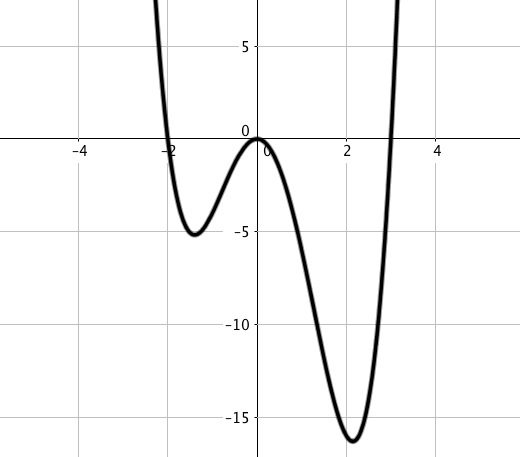
\includegraphics[width=0.8\textwidth]{img2/sol-bloc2-polinomi1.png}
	\end{minipage}

	
	\item \begin{minipage}[t]{0.5\textwidth}
		\begin{tasks}(1)
				\task $y=1$ asímptota horitzontal; $x=1$ i $x=3$ asímptotes verticals. La posició relativa és: $\limx{+\infty} f(x)=1$ per damunt; 
				$\limx{-\infty} f(x)=1$ per davall. $\limx{1^-} f(x)=+\infty$, $\limx{1^+} f(x)=-\infty$, $\limx{3^-} f(x)=-\infty$, $\limx{3^+} f(x)=+\infty$.
				%
				\task La funció té un mímim relatiu a $x=0$, $y=0$ i un màxim relatiu a $x=3/2$, $y=-3$
				%
		\end{tasks}
	\end{minipage}
		\begin{minipage}[t]{0.5\textwidth}
		  \begin{center}
		c) Gràfica: 	
		
		\includegraphics*[width=0.8\textwidth]{img2/bloc2-10.png}
		\end{center}
	\end{minipage}
	
	\item $k=1/2$. La primera derivada $y'=(2x^2+2x+1)/(x+1/2)^2$ mai és zero. Sempre creix i per tant no té extrems.
	
	
	\item \begin{minipage}[t]{0.5\textwidth}L'única funció que presenta asímptota obliqua és c). L'asímptota obliqua és $y=2x+2$ i també té una asímptota vertical a $x=1$. La gràfica és la següent:
		\end{minipage}
	\begin{minipage}[c]{0.5\textwidth}
	\begin{center}
	\includegraphics*[width=0.7\textwidth]{img2/bloc2-11.png}
	\end{center}
	\end{minipage}

	\item $a=-6$ i $b=17$. 
	
\end{enumerate}


%%%%%%%%%%%%%%%%%%%%%%%%%%%%%%%%%%%%%%%%%%%%%%%%%%%%%%%%%


\section*{TEMA \ref{chap:vectors}: \nameref{chap:vectors}}

\subsection*{Solucions de l'autoavaluació}
\begin{enumerate}
	\item a) Punt final $(-3,2)$. b) Vector suma $\vvec+\vec w=(-2,3)$.
	\item a) $-3$.  b) $-11$
	\item a) $2\sqrt{3}$. b) Els dos tenen mòdul 2. c) angle $30^\circ$
	\item a) $k=-2$. b) $k=\pm 4$. c) $k=-\sqrt{3}$
	\item $()$
\end{enumerate}


%%%%%%%%%%%%%%%%%%%%%%%%%%%%%%%%%%%%%%%%%%%%%%%%%%%%%%%%%%%%%%%%%%%%%%%%%%%%%%%%%%%%%%%%%%%%%%%%%%%%%%%%%%%%%%%%%%





\section*{TEMA \ref{chap:analitica}: \nameref{chap:analitica}}

\subsection*{Solucions de l'autoavaluació}
\begin{enumerate}
	\item a) $k=-7$, b) $k=-7$
	\item Contínua $\frac{x-3}{5}=\frac{y-2}{1}$, general $x-5y+7=0$.
	\item a) $(x,y)=(2,-3)+\lambda(2, 5)$,  b) $2x+3y-6=0$.
	\item Si $k=-9/5$ són paral·leles, en altre cas són secants.
	\item $k=\pm \sqrt{3}$.
\end{enumerate}


%%%%%%%%%%%%%%%%%%%%%%%%%%%%%%%%%%%%%%%%%%%%%%%%%%%%%%%%%%%%%%%%%%%%%%%%%%%%%%%%%%%%%%%%%%%%%%%%%%%%%%%%%%%%%%%%%%


\section*{TEMA \ref{chap:coniques}: \nameref{chap:coniques}}

\subsection*{Solucions de l'autoavaluació}

\begin{enumerate}
\item $x^2+y^2-2x-2y-23=0$ o $(x-1)^2+(y-1)^2=25$. Té centre $O(1,1)$ i radi $R=5$.

\item $\frac{(x+1)^2}{25}+\frac{(y-3)^2}{9}=1$. La semi-distància focal $c=4$, els focus són $F'(-5,3)$ i $F(3,3)$, i l'excentricitat $e=0.8$.

\item Semi-eixos: $a=2$, $b=\sqrt{2}$, les asímptotes $y=\pm\frac{\sqrt{2}}{2}x$, semi-distància focal: $c=\sqrt{6}$ l'excentricitat $e=1.225$.

\item La distància focus-directriu és $p=1/6$, l'equació $y-2=3 (x-1)^2$, la directriu és la recta $y=23/12$ i la posició del focus $F(1, 25/12)$.

\item a) El·lipse de centre $(1,0)$ i semi-eixos $a=2$, $b=1$.  b) Circumferència de centre $(1,2)$ i radi $2$. c) Paràbola vertical de vèrtex $(0,-2)$ i distància Focus-directriu $p=3/2$.
\end{enumerate}


%%%%%%%%%%%%%%%%%%%%%%%%%%%%%%%%%%%%%%%%%%%%%%%%%%%%%%%%%%%%%%%%%%%%%%%%%%%%%%%%%%%%%%%%%%%%%%%%%%%%%%%%%%%%%%%%%%


\section*{SÍNTESI DE LA PART III - Geometria en el pla}
\begin{enumerate}
	
	\item a) $|\vec u|=\sqrt{2}$
  	  	 b) $-2\vec u + 3\vvec=(-5,-4)$
  		 c) $2\vec u \cdot (\vec u + \vvec)=6$
  		 
 	\item $a=-2$ 	
 	
 	\item a) $m=-1$, $n=3$   b) $116.57^\circ$
 	
 	\item $(\frac{1}{2}, \frac{\sqrt{3}}{2})$
 	
 	\item $y=-8$
 	
 	\item Paramètriques $\left\{\begin{array}{l} x=0+1t \\ y=3+2t \end{array}\right.$. General $2x-y-3=0$.
 	
 	\item a) $k=-2$.  b) $k=-4$
 	
 	\item $A'(2,2)$
 	
 	\item El punt d'intersecció és $I(5,11)$ i el pendent de la recta $m'=1/3$. La recta és $y-11=\frac{1}{3}(x-5)$.
 	
 	\item $P(\pm 5, 0)$
 	
 	\item $Area=5$
 	
 	\item  Centre $O(1,-3)$ i radi $R=2$.
 	
 	\item $\frac{x^2}{100}+\frac{y^2}{36}=0$
 	
 	\item 
 	 
 		a) Paràbola vertical amb vèrtex $V(0,0)$, $p=3$, focus $F(0,3/2)$ i directriu la recta $y=-3/2$.
 	
 		b) Hipèrbola de centre $O(1,-1)$, semieixos $a=4$, $b=3$, semi-distància focal $c=5$. Excentricitat $e=1.25$. Focus a $F'(-4,-1)$, $F(6,-1)$. Asímptotes $y+1=\pm\frac{3}{4}(x-1)$.

 		\begin{center}
 			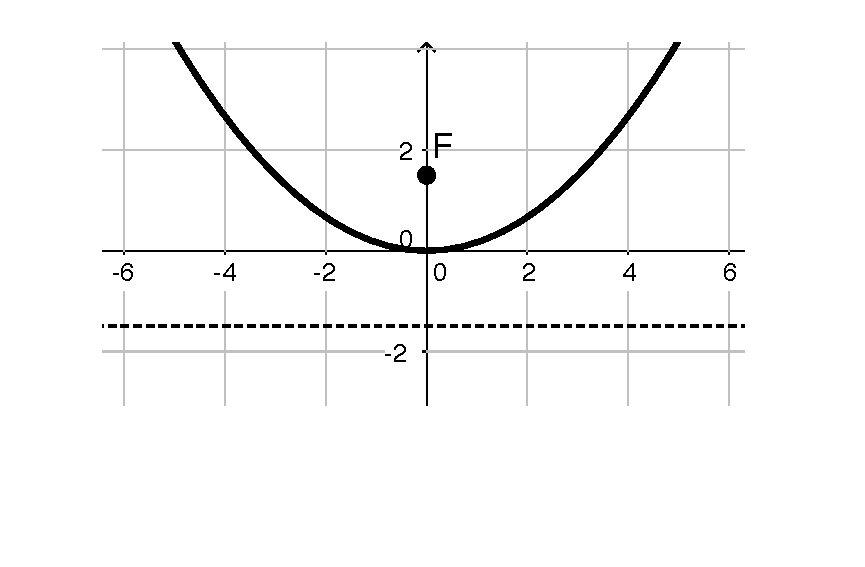
\includegraphics[height=3.4cm]{img2/bloc3-sol-14a}
 			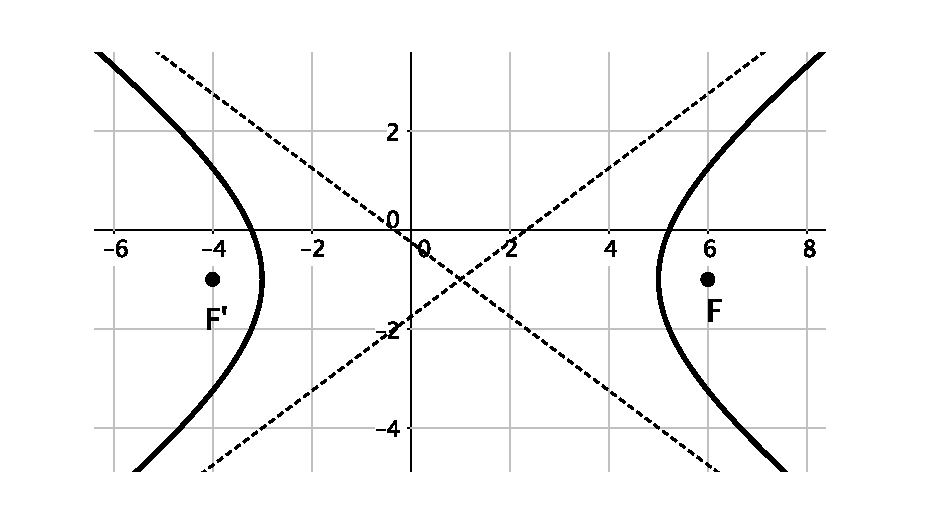
\includegraphics[height=3.4cm]{img2/bloc3-sol-14b}
 		\end{center}
  
\end{enumerate}



\section*{TEMA \ref{chap:estadistica}: \nameref{chap:estadistica}}

\subsection*{Solucions de l'autoavaluació}

\begin{enumerate}
	\item \begin{minipage}{0.7\textwidth} a) Hi ha una correlació positiva i forta entre les variables. El coeficient de correlació és $r=0,91$  b) La recta de regressió és $y=0.87x+2.25$. \end{minipage}
	\begin{minipage}{0.3\textwidth}
		\includegraphics[width=0.8\textwidth]{img2/chap-est-aval1}
		\end{minipage}
	 
	
		\item \begin{minipage}{0.7\textwidth} El pes i la talla estan relacionats mitjançant una correlació feble positiva. La covariància és $\sigma_{xy}=3.55$, el coeficient de correlació $r=0.54$ i la recta de regressió $y=69+3,38(x-41,45)$ \end{minipage}
	\begin{minipage}{0.3\textwidth}
		\includegraphics[width=0.8\textwidth]{img2/chap-est-aval2}
	\end{minipage}

		\item a) $y=0,0989 x + 6,65$. b) $r=0.16$ pràcticament no hi ha correlació. Les prediccions amb la recta de regressió no són fiables.
\end{enumerate}